\documentclass[11pt,a4paper]{article}
\usepackage[T1]{fontenc}
\usepackage{lmodern,microtype}
\usepackage{amsmath,amssymb,amsthm,mathtools}
\usepackage{geometry,booktabs,hyperref,tikz}
\usetikzlibrary{arrows.meta}
\geometry{margin=27mm}
\hypersetup{colorlinks=true,linkcolor=blue,urlcolor=blue}
\newtheorem{theorem}{Theorem}[section]
\newtheorem{lemma}[theorem]{Lemma}
\newtheorem{proposition}[theorem]{Proposition}
\newtheorem{remark}[theorem]{Remark}
\newcommand{\Rzero}{R_0}
\title{An Exact Computer-Assisted Optimality Certificate\\for Nine Disks of Radii $1,2,\ldots,9$}
\author{Independent research draft}
\date{October 9, 2026}
\begin{document}
\maketitle
\begin{abstract}
We give an exact, independently replayable computer-assisted argument for the minimum radius of a circular container accommodating disks of radii $1,2,\ldots,9$.  The claimed optimum is the unique root of a six-angle closure equation near $19.23319390808612$. An explicit construction proves attainability. The global lower bound reduces to an exhaustive rational radial tree with 47 nodes: 23 leaves reject all sixty cyclic orders using negative cycles in angle-difference constraints; the final leaf rejects fifty-nine orders by negative cycles and the remaining order by a strict radial monotonicity argument. The decisive replay checks use integer and rational arithmetic, not floating-point arithmetic. This is a computer-assisted draft, not a formal theorem-prover development or a peer-reviewed result.
\end{abstract}

\section{Problem and exact statement}
Let $D_i$ be a disk of radius $i$ with center $p_i\in\mathbb R^2$, $1\le i\le9$. For a container centered at the origin, feasibility at radius $R$ means
\begin{equation}\label{eq:feasibility}
\|p_i\|+i\le R,\qquad\|p_i-p_j\|\ge i+j\quad (i\ne j).
\end{equation}
For $R>i+j$ define the angle between two wall-tangent, mutually tangent disks by
\begin{equation}\label{eq:beta}
\beta_{ij}(R)=2\arcsin\sqrt{\frac{ij}{(R-i)(R-j)}}.
\end{equation}
Let $C=(9,5,7,6,8,4)$, with consecutive pairs interpreted cyclically, and set
\begin{equation}\label{eq:closure}
\begin{aligned}
H(R)={}&\beta_{95}(R)+\beta_{57}(R)+\beta_{76}(R)\\
&+\beta_{68}(R)+\beta_{84}(R)+\beta_{49}(R)-2\pi.
\end{aligned}
\end{equation}
Write $\Rzero$ for the unique zero of $H$ in the rational interval
\begin{equation}\label{eq:root-box}
J_R=[19.23319390808612,\;19.23319390808613].
\end{equation}
The exact root is strictly less than the rational tree cap
\begin{equation}\label{eq:U}
 U=19.23319390809.
\end{equation}
\begin{theorem}[Global optimality]\label{thm:main}
The minimum possible container radius for nine nonoverlapping disks of radii $1,2,\ldots,9$ is exactly $\Rzero$.
\end{theorem}
The displayed decimals in \eqref{eq:root-box} and \eqref{eq:U} are terminating decimal fractions and hence exact rationals. They are not definitions by numerical approximation.

\section{Exact upper bound: a nine-disk witness}
\begin{lemma}[Existence and uniqueness of the critical radius]\label{lem:root}
The function $H$ has precisely one zero in $J_R$, and $\Rzero<U$.
\end{lemma}
\begin{proof}
All six angles are defined for $R\in J_R$, because $R>17$ there. Their derivatives satisfy
\[
\beta_{ij}'(R)=-\left(\frac1{R-i}+\frac1{R-j}\right)\tan\frac{\beta_{ij}(R)}2<0.
\]
An exact rational interval evaluation of square roots, arctangents, and $\pi$ certifies $H(\inf J_R)>0$ and $H(\sup J_R)<0$; see the accompanying verifier \texttt{verify\_nine\_upper.py}. Continuity and strict monotonicity imply the assertion. The upper endpoint of $J_R$ is smaller than $U$.
\end{proof}

For each $i\in C$ set $s_i=\Rzero-i$. Start with disk $9$ at
\[
p_9=(\Rzero-9,0).
\]
Place the remaining core disks counterclockwise in the order $9,5,7,6,8,4$, with each successive angular gap equal to the corresponding $\beta_{ij}(\Rzero)$. Equation \eqref{eq:closure} closes this six-disk ring. All core disks touch the container and every cyclic neighboring pair is tangent.

Place the three other disk centers at the following \emph{exact rational} coordinates:
\begin{equation}\label{eq:smallcenters}
  p_1=(-14.16,-11.20),\quad
  p_2=(13.7125,-10.4353),\quad
  p_3=(-3.94,0.45).
\end{equation}
The rational interval verifier evaluates the core centers over the full root interval $J_R$. It proves that the other $\binom92-6=30$ pairs have strictly positive squared nonoverlap slack, and that disks $1,2,3$ lie strictly inside the container. The six core tangencies are consequences of the exact angular definitions and closure, not approximate numerical contacts.
Therefore
\begin{equation}\label{eq:upper}
R^*\le\Rzero.
\end{equation}

\begin{figure}[htbp]\centering
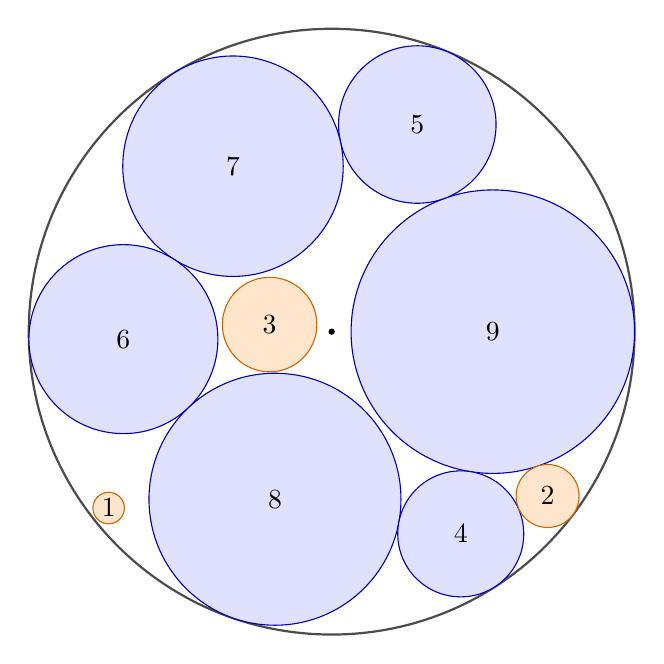
\begin{tikzpicture}[scale=.20]
 \draw[black!70,thick] (0,0) circle (19.233194);
 \foreach \x/\y/\r/\id in {
10.23319/0/9/9,5.43829/13.15328/5/5,-6.26618/10.50648/7/7,
-13.22469/-.47437/6/6,-3.59958/-10.64085/8/8,8.19727/-12.83959/4/4} {
  \draw[draw=blue!70!black,fill=blue!12] (\x,\y) circle (\r);
  \node[font=\normalsize] at (\x,\y) {$\id$};
 }
 \foreach \x/\y/\r/\id in {-14.16/-11.20/1/1,13.7125/-10.4353/2/2,-3.94/.45/3/3} {
   \draw[draw=orange!80!black,fill=orange!20] (\x,\y) circle (\r);
   \node[font=\normalsize] at (\x,\y) {$\id$};
 }
 \fill (0,0) circle (.2);
\end{tikzpicture}
\caption{Illustrative nine-disk witness. The blue disks $4,5,6,7,8,9$ form a wall-tangent six-cycle. Coordinates in the illustration are rounded; the proof uses the exact angle-root construction and the rational auxiliary centers \eqref{eq:smallcenters}.}\label{fig:witness}
\end{figure}

\section{Angle constraints on radial boxes}
We prove the lower bound for all placements of just the six largest disks $4,\ldots,9$. Let $s_i=\|p_i\|$. From containment and the triangle inequality, every packing with $R\le U$ obeys
\begin{equation}\label{eq:initialbox}
\ell_i=\max\left\{0,\max_{\substack{j\in\{4,\ldots,9\}\\j\ne i}}(i+2j-U)\right\}\le s_i\le U-i=u_i.
\end{equation}
Every $\ell_i$ is positive. If a radial box is $s_i\in[\ell_i,u_i]$, the pairwise inequality $s_i+s_j\ge i+j$ permits sound propagation of its lower endpoints.

\begin{lemma}[Four-corner radial-cosine bound]\label{lem:corner}
For $d>0$ and a rectangle $[a,b]\times[c,e]\subset(0,\infty)^2$, the function
\[
K_d(x,y)=\frac{x^2+y^2-d^2}{2xy}
\]
attains its maximum at a corner.
\end{lemma}
\begin{proof}
For fixed $y$, $\partial K_d/\partial x=(x^2-y^2+d^2)/(2yx^2)$. Any interior critical point is a minimum, so the maximum over $x$ is at an endpoint. The same argument on either resulting edge applies to $y$.
\end{proof}

The law of cosines gives a necessary smaller angular separation between the two center rays:
\begin{equation}\label{eq:phi}
\phi_{ij}(s_i,s_j)=\arccos K_{i+j}(s_i,s_j).
\end{equation}
By Lemma~\ref{lem:corner}, a proposed rational angular lower bound $q_{ij}\ge0$ is sound whenever
\begin{equation}\label{eq:tick}
C_{18}(q_{ij})\ge\max_{x\in\{\ell_i,u_i\},\;y\in\{\ell_j,u_j\}} K_{i+j}(x,y),
\end{equation}
where $C_{18}$ is the degree-18 Taylor polynomial for cosine, satisfying $C_{18}(q)\le\cos q$ for $0\le q\le\pi$. The verifier checks \eqref{eq:tick} exactly with rational arithmetic.

After orienting and lifting a cyclic order $(i_0,\ldots,i_5)$ of the six center rays, every $a<b$ must satisfy
\begin{equation}\label{eq:diff}
q_{i_ai_b}\le\theta_b-\theta_a\le2\pi_+-q_{i_ai_b},
\qquad \pi<\pi_+=3.141592653590.
\end{equation}
\begin{lemma}[Negative-cycle exclusion]\label{lem:cycle}
A collection of necessary inequalities $\theta_v-\theta_u\le w_{uv}$ is infeasible if its directed graph contains a cycle of strictly negative total weight.
\end{lemma}
\begin{proof}
The inequalities telescope on a directed cycle to $0\le\sum w_{uv}<0$.
\end{proof}

\section{The finite lower-bound certificate}
A six-element labeled cyclic order has $5!/2=60$ representatives modulo rotation and reflection. We root each order at disk $9$ and fix a representative orientation. Reflections preserve the radial constraints and distances, hence no configuration is lost.

The certificate begins at the full box \eqref{eq:initialbox}. Each internal node bisects one radial interval at an exact rational cut, and the two closed children cover the parent. A leaf either excludes all 60 orders by explicit negative cycles in \eqref{eq:diff}, or records negative cycles for 59 orders and applies the following analytic barrier to the last order.

\begin{lemma}[Local wall-angle barrier]\label{lem:barrier}
Let $C=(9,5,7,6,8,4)$. Suppose a radial box with lower endpoints $\ell_i$ has, for each successive pair $i,j$ of $C$, the inequalities
\begin{align*}
\ell_i+\ell_j&>i+j,\\
\max\{|\ell_i-(U-j)|, |(U-i)-\ell_j|\}&<i+j,\\
\ell_i^2-(U-j)^2+(i+j)^2&>0,\\
\ell_j^2-(U-i)^2+(i+j)^2&>0.
\end{align*}
If a packing in that box exists with container radius $17<R<\Rzero$, then its six largest center rays cannot have cyclic order $C$ or its reverse.
\end{lemma}
\begin{proof}
Differentiation of \eqref{eq:phi} gives, where $0<\phi_{ij}<\pi$,
\[
\frac{\partial\phi_{ij}}{\partial s_i}
=-\frac{s_i^2-s_j^2+(i+j)^2}{2s_i^2s_j\sin\phi_{ij}}.
\]
The hypotheses guarantee that the derivative with respect to either radial coordinate is strictly negative throughout the extension of the box to $[\ell_i,U-i]$ for each disk. The strict triangle inequalities keep the angles well-defined throughout the comparison. Replacing the six radial coordinates by their wall values $R-i$ \emph{only in the angle formulas}, without moving the physical disks, shows
\[
2\pi\ \ge\ \sum_{(i,j)\in C}\phi_{ij}(s_i,s_j)
\ \ge\ \sum_{(i,j)\in C}\beta_{ij}(R)
\ >\ \sum_{(i,j)\in C}\beta_{ij}(\Rzero)=2\pi,
\]
a contradiction. The final strict inequality uses $R<\Rzero$ and the strict decrease of the functions $\beta_{ij}$ in $R$.
\end{proof}

\begin{proposition}[Verified finite cover]\label{prop:certificate}
The accompanying exact rational checker verifies that the 47-node radial tree covers the initial box \eqref{eq:initialbox}. Every leaf is excluded for hypothetical packings with $R<\Rzero$ by Lemma~\ref{lem:cycle} or Lemma~\ref{lem:barrier}.
\end{proposition}
\begin{proof}
The replay reconstructs every interval from the root and exact rational child cuts; it never treats the recorded leaf boxes as independent assumptions. Every integer angle tick is checked by \eqref{eq:tick}. Each listed directed negative cycle is checked for consecutive edge endpoints, use of the correct constraints, absence of duplicated vertices, and a strictly negative rational weight sum. At the unique barrier leaf, the checker recomputes all four families of inequalities in Lemma~\ref{lem:barrier}, and proves $s_9+9>17$ for every point of that leaf. The checker checks the entire original set of 60 orders at each leaf, and the full binary-tree identity. The resulting ledger is shown in Table~\ref{tab:tree}.
\end{proof}
\begin{table}[htbp]\centering
\caption{Rational proof-tree replay for disks $4,\ldots,9$.}\label{tab:tree}
\begin{tabular}{lr}\toprule
Nodes & 47\\
Rational splits & 23\\
Leaves & 24\\
Negative-cycle leaves (all 60 orders) & 23\\
Barrier leaves (59 cycles and 1 analytic barrier) & 1\\
Maximum tree depth & 14\\
Unresolved leaves & 0\\
\bottomrule\end{tabular}
\end{table}
The minimum rational negative-cycle margin in the checked file is
\[
\frac{974034641}{50000000000}>0.
\]
For the barrier leaf, the radial lower endpoints (shown in decimal for readability; exact fractions appear in the certificate) satisfy
\begin{center}\small
\begin{tabular}{ccc}\toprule
Disk $i$ & Certified lower endpoint $\ell_i$ & Upper endpoint $U-i$\\\midrule
4 & 13.6748954310675 & 15.23319390809\\
5 & 12.9248954310675 & 14.23319390809\\
6 & 11.1165969540450 & 13.23319390809\\
7 & 10.6165969540450 & 12.23319390809\\
8 & 10.1165969540450 & 11.23319390809\\
9 & 9.1165969540450 & 10.23319390809\\
\bottomrule
\end{tabular}
\end{center}

\begin{proof}[Proof of Theorem~\ref{thm:main}]
By Lemmas~\ref{lem:corner}, \ref{lem:cycle}, and \ref{lem:barrier} and Proposition~\ref{prop:certificate}, no six disks of radii $4,\ldots,9$ fit in a container of radius $R<\Rzero$. Hence no packing of all nine disks exists below $\Rzero$. Lemma~\ref{lem:root} and the explicit nine-disk construction establish feasibility at $\Rzero$, proving $R^*=\Rzero$.
\end{proof}

\section{Reproducibility and limitations}
The full replay is available in the accompanying files. Run
\begin{quote}\small\ttfamily
python3 certify\_integer\_nine\_global.py
\end{quote}
The dispatcher runs the exact root/upper-bound witness checker and the independent exact rational lower-bound tree checker. The generator \texttt{gen\_nine\_global\_tree.py} uses floating point only to \emph{discover} possible angle ticks and branch structure; it is not needed for replay. All decisive verifier tests use exact integers and Python \texttt{Fraction}, with outward integer-square-root intervals and rational Taylor/arctangent bounds. The Python implementation and interpretation of the finite certificate remain part of the trust base; the proof has not been independently formalized in a theorem prover or peer reviewed.

The numerical value of the optimum agrees with the best-known nine-disk arrangement listed by Packomania, \url{https://www.packomania.com/ccin/}. Establishing whether an identical proof has appeared elsewhere requires a separate priority search.
\end{document}
